\subsubsection{I fenomeni più importanti}

Per quanto riguarda il continuo, i processi che contribuiscono maggiormente all'opacità sono

\begin{itemize}
  \item Fotoionizzazione dell'atomo di Idrogeno; un atomo di Idrogeno che si trova in un livello legato assorbe un fotone e viene così ionizzato. Un tale processo può essere schematizzato come una “reazione” del tipo $\rm H + h \nu \ce{->} H^+ + e^-$;
  \item Fotoionizzazione dello ione negativo di Idrogeno: $\rm H^- + h \nu \ce{->} H + e^-$;
  \item Scattering Thomson.
\end{itemize}

A questo punto ci si potrebbe chiedere se quando abbiamo espresso la classificazione delle stelle in termini di presenza o assenza di righe spettrali, questo ragionamento possa essere esteso all'andamento del cosiddetto continuo, che è determinato dall'interazione radiazione-materia in quei processi dove l'energia dei fotoni non è strettamente determinata (ad esempio la ionizzazione o la diffusione: c'è un valore di soglia al di sotto del quale non avvengono, ma poi avviene per tutti i valori più alti). In realtà lo abbiamo in qualche modo fatto perché abbiamo detto che la presenza o meno delle discontinuità (che sono un prodotto della ionizzazione) è una conferma dei processi atomici; inoltre l'ampiezza di una discontinuità c'entra con la ionizzazione degli atomi, quindi sull'intensità delle righe spettrali.

Vediamo di estendere questo concetto, chiedendoci se il continuo è esso stesso indicatore della temperatura o se il comportamento del continuo dipende dalla temperatura. Questo è un concetto importante perché la possibilità di determinare la temperatura sulla base delle righe spettrali, prevede che si possano osservare le righe spettrali, il che non è detto a priori. Immaginiamo, ad esempio, di dover determinare la presenza di una riga spettrale di una stella con una magnitudine molto alta (uguale a zero): ci sarà un numero di fotoni al secondo dell'ordine di grandezza di 1000 per $\rm cm^2$. Ricordiamo, inoltre, che il rapporto segnale-rumore è uguale a $\sqrt{n}$, con $n$ numero di fotoni, in questo caso circa uguale a 30. La capacità di vedere la riga o meno dipende da vari fattori, ad esempio dalle caratteristiche dello strumento utilizzato. Se adesso immaginassimo di avere una stella di sedicesima magnitudine, il numero di fotoni si riduce a meno 1.

Così come per le righe spettrali non ci interessano tutti i livelli spettrali di un atomo e tutti gli elementi, lo stesso vale per il continuo. Una fonte di continuo che si può considerare, per esempio, nel caso del Sole, è l'idrogeno $\rm H^-$. Infatti, nel caso del Sole, l'ambiente è freddo (5800 K, che per le stelle sono bassi) e a queste temperature l'Idrogeno si ionizza poco, però si ionizzano molto i metalli, il cui potenziale di ionizzazione è dell'ordine di pochi eV. Di conseguenza, l'Idrogeno neutro potrebbe catturare molti elettroni, dando vita all'Idrogeno negativo $\rm H^-$. Quest'ultimo si occupa di fermare sostanzialmente tutti i fotoni (quelli con $\lambda < 1.65 \; \mu$m), che hanno un'energia superiore a quella del bassissimo potenziale di ionizzazione dell'Idrogeno negativo, pari a 0.754 eV. Ne segue che lo spettro del Sole viene prodotto dall'interazione di tutti i fotoni che si trovano all'interno, perché tutti hanno energia sufficiente a strappare l'elettrone all'$\rm H^-$. Questo vuol dire che nelle stelle più fredde, come il Sole, l'Idrogeno negativo diventa la prima forma di ionizzazione e quindi di continuo. A questa forma di opacità contribuiscono tanti elementi, ma quello che riguarda l'$\rm H^-$ risulta particolarmente dominante. Quello che è interessante notare è che la probabilità di assorbimento ha un andamento in funzione della lunghezza d'onda che, tutto sommato, in gran parte dello spettro si potrebbe considerare quasi constante.

\begin{figure}[H]
  \centering
  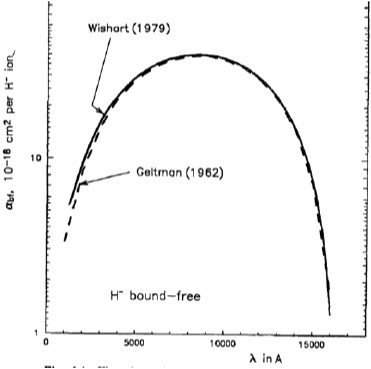
\includegraphics[width=7cm]{Hcontinuo.jpg}
  \label{fig:Hcontinuo}
\end{figure}

(In figura: Andamento della probabilità di assorbimento in funzione della lunghezza d'onda.)

Naturalmente ci sono tante altre molecole che si possono formare e, paradossalmente, nelle stelle più fredde si forma anche l'acqua. Tuttavia questa, che si trova ad una temperatura di circa 5000 K, non si deve immaginare come l'acqua che conosciamo noi, ma è come una coincidenza in un luogo di due Idrogeni e di un Ossigeno che in quel momento sono così vicini da dare vita ai legami tipici di una molecola (che poi si dissolve subito, ma visto che l'ambiente ne è pieno si riformano altre molecole). Il fatto che questi modelli tengano conto anche delle molecole è molto recente ed è una scoperta molto importante in quanto l'opacità dell'acqua (che è enorme, basti pensare alle nuvole) è importante per fare un buon modello del comportamento della radiazione.

Un altro fenomeno interessante di scattering è quello tra la radiazione e gli elettroni liberi. La probabilità di interazione tra un campo elettromagnetico e un elettrone, indipendente dalla lunghezza d'onda, è molto bassa (si ha una sezione d'urto $\rm \sigma_T= 6.65 \cdot 10^{-25}cm^2$). Tuttavia le densità sono molto alte e, se ci sono tanti elettroni liberi, come ad esempio nelle regioni intorno al Sole nella cosiddetta \textit{corona solare}\footnote{Noi vediamo, ad esempio attraverso sonde, gli elettroni liberi che si trovano intorno al Sole perché la radiazione di questo viene riflessa dagli elettroni nella direzione della Terra.}, lo Scattering Thomson avviene. Esso è un fenomeno in cui un fotone, generalmente di luce visibile o raggi X, interagisce con una particella carica. In esso non vi è assorbimento di energia da parte della particella, e quindi l'energia del fotone non cambia dopo l'interazione; il risultato principale è una deviazione della direzione di propagazione del fotone in seguito all'interazione con la particella. Questo tipo di scattering è molto interessante perché, essendo indipendente dalla lunghezza d'onda, se osservato, fornisce immediatamente la densità degli elettroni (ad esempio, se guardiamo la percentuale di radiazione scatterata dal Sole nella nostra direzione, possiamo dire come gli elettroni sono distribuiti attorno ad esso).

Nel caso più generale dobbiamo tenere in considerazione tutti i fenomeni che conosciamo, che sostanzialmente sono tre: ionizzazione dell'Idrogeno, ionizzazione dell'$\rm H^-$ e Scattering Thomson. Questi tre processi avvengono tutti contemporaneamente e, a seconda della temperatura delle stelle, sono più o meno dominanti: nelle stelle fredde (ad esempio il Sole) il continuo è determinato dalla ionizzazione dell'Idrogeno negativo

\begin{figure}[H]
  \centering
  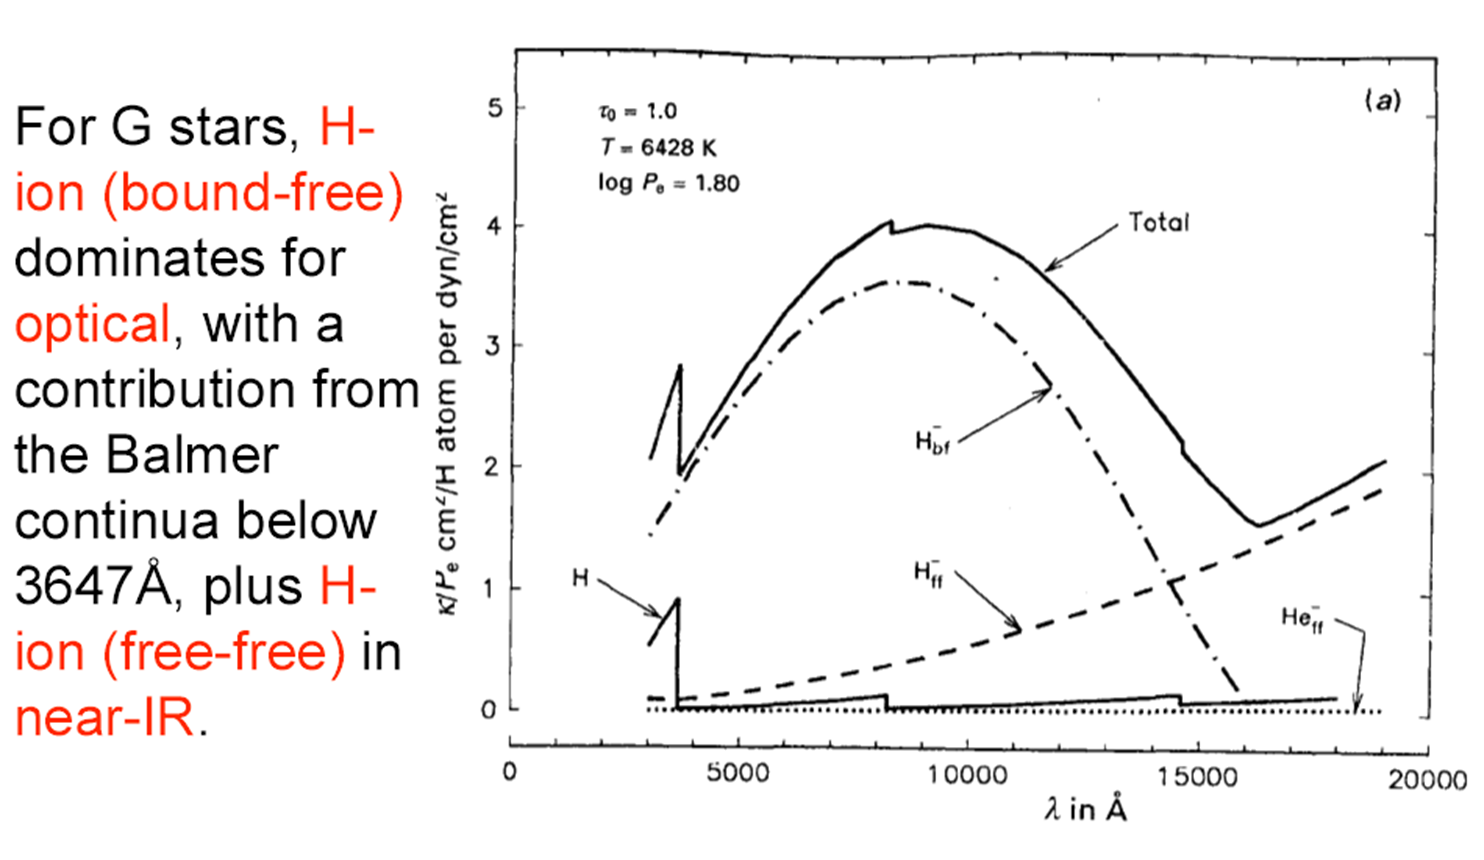
\includegraphics[width=10cm]{immagini/spettro_stelle_solari.png}
\end{figure}

nelle stelle di tipo A è dominante la ionizzazione dell'Idrogeno con le varie discontinuità di Balmer, Paschen ecc.

\begin{figure}[H]
  \centering
  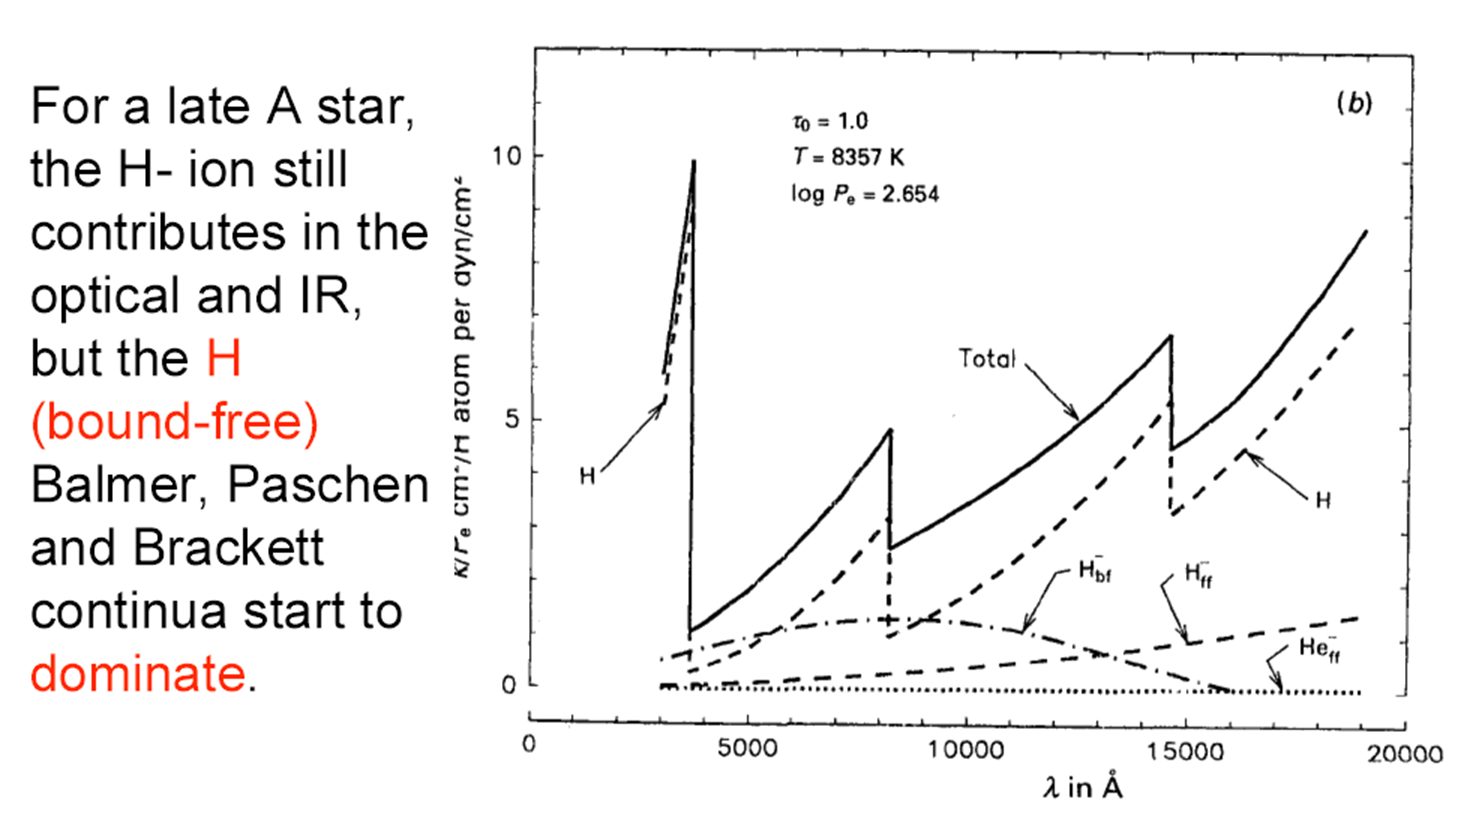
\includegraphics[width=10cm]{immagini/spettro_stelle_A.png}
\end{figure}

Infine nelle stelle più calde, dove c'è maggiore ionizzazione e quindi molti elettroni liberi, è dominante lo scattering Thomson

\begin{figure}[H]
  \centering
  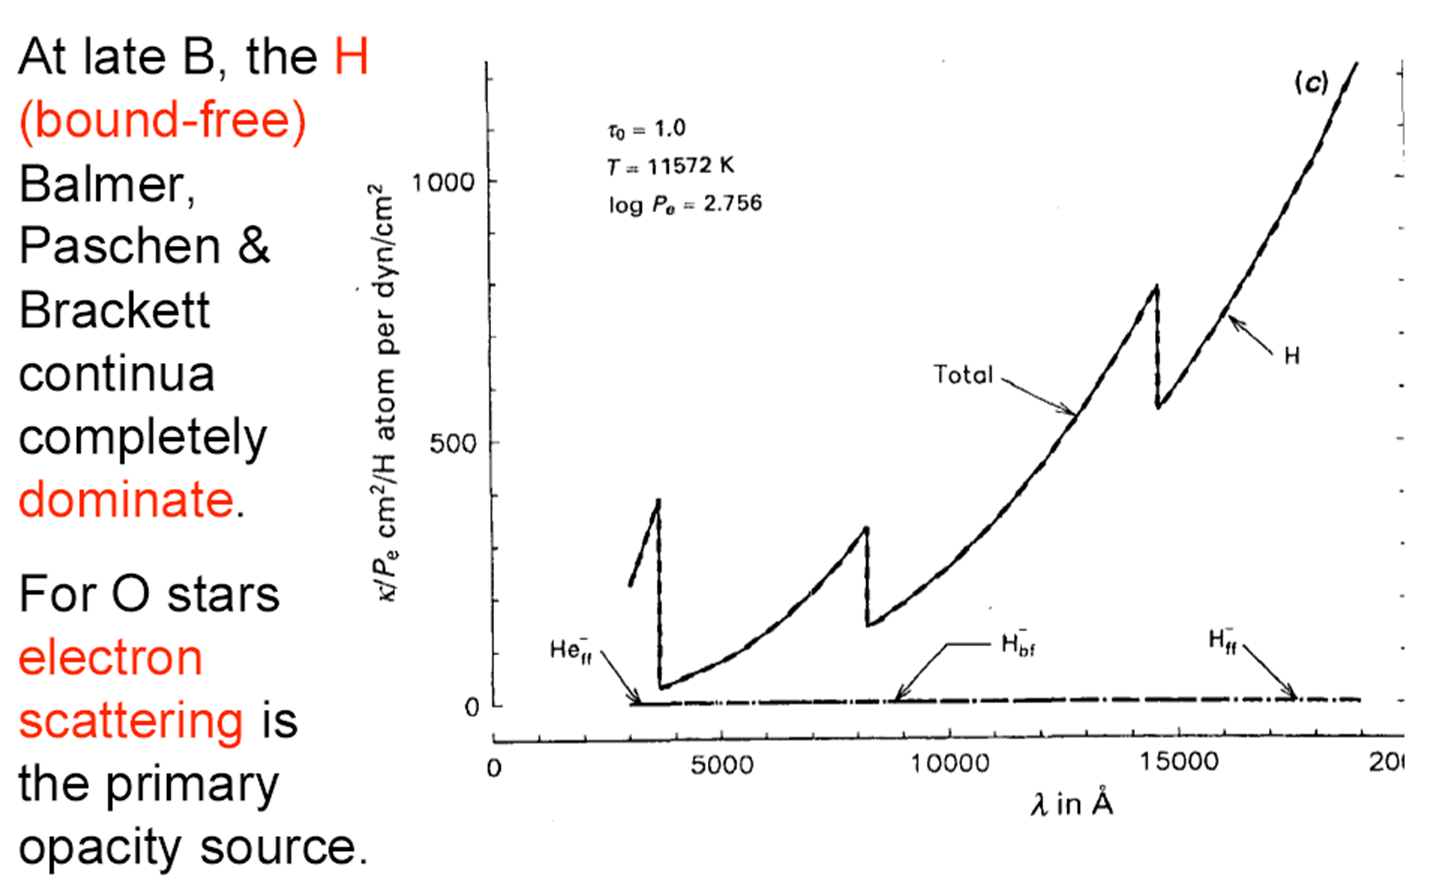
\includegraphics[width=10cm]{immagini/spettro_stelle_calde.png}
\end{figure}


Ora si comprende meglio la forma degli spettri, infatti, per le stelle di tipo O non c'è ionizzazione, si ha solo l'andamento del corpo nero, lo scattering è indipendente dalla lunghezza d'onda e quindi non cambia la sua forma. Quando la temperatura si abbassa si ha la ionizzazione dell'Idrogeno, quindi al corpo nero bisogna sottrarre l'andamento di ionizzazione, che è fatto di salti. Nelle stelle più fredde, infine, dove è predominante la ionizzazione dell'$\rm H^-$ , lo spettro presenta un picco nelle regioni di lunghezza d'onda maggiore. Il fatto che i due processi appena visti sono molto poco dipendenti dalla lunghezza d'onda permette di risolvere l'equazione del trasporto radiativo per una sola lunghezza d'onda.

\subsubsection{Polarizzazione. Parametri di Stokes}
I processi appena analizzati, soprattutto lo scattering Thomson, sono capaci di polarizzare la radiazione. Le informazioni sulla polarizzazione sono utilissime per sapere se una stella ha un disco o per determinare l'esistenza di un pianeta\footnote{dato che ci aspettiamo che il pianeta orbiti intorno alla stella presa in considerazione, la polarizzazione dovrebbe cambiare continuamente.}. Immaginiamo, ad esempio, di vedere, tramite dei satelliti, la luce del Sole riflessa dalla Terra nello spazio: il grado di polarizzazione che il satellite vede guardando la Terra dipende, ad esempio, da cosa sta guardando (mare, montagne, vegetazione). Infatti, il più alto grado di polarizzazione si ha quando la luce viene riflessa dall'acqua, mentre quando si guarda una foresta si avrà una polarizzazione circolare, indotta dalle foglie.

Per la misura del grado di polarizzazione di una radiazione è necessario un sistema di riferimento. Questa consiste nella misura del campo elettrico in due direzioni ortogonali che rappresentano il nostro sistema di riferimento. Ad esempio si può considerare il caso ideale in cui $E_x=0$ e $E_y$ varia continuamente: non possiamo misurare $E_x$ o $E_y$, ma solo il modulo quadro perché le variazioni del campo elettrico, ad esempio nel visibile, sono troppo veloci per gli strumenti attualmente a disposizione (invece nel caso delle onde radio si possono misurare le variazioni anche banalmente con il telefono). La misurazione del campo elettrico in due stati di polarizzazione ortogonali si può fare con una banale calcite che, quando arriva il fascio di luce, lo separa in un fascio ordinario (ovvero il fascio polarizzato in un certo modo) e il fascio polarizzato ortogonalmente. Quindi, un po' come avviene per la spettroscopia, si separano la $x$ dalla $y$ e si fanno due misure diverse.

Per una descrizione completa del tipo di polarizzazione vengono utilizzati i parametri di Stokes

\begin{equation}
  \begin{cases}
    I={E_{0x}^2} + {E_{0y}^2}\\
    Q={E_{0x}^2} - {E_{0y}^2}\\
    U=2E_{0x}E_{0y} \cos(\delta_1 - \delta_2)\\
    V=2E_{0x}E_{0y} \sin(\delta_1 - \delta_2)\\
  \end{cases}
\end{equation}

dove $\delta_1$ e $\delta_2$ sono gli angoli di polarizzazione.

Il parametro $I$ indica l'intensità della radiazione, $Q$ ci dà un'informazione su quanto sono diverse la $E_{0x}^2$ e la $E_{0y}^2$. Dopodiché si può provare a vedere se esiste uno stato di polarizzazione in una direzione diversa e definire un nuovo parametro $U$ che ci dice com'è polarizzata la radiazione a 45° rispetto al sistema di riferimento. Infine $V$ ci dice se il vettore di polarizzazione sta compiendo un cerchio. 

\begin{minipage}{0.395\textwidth}
  \begin{figure}[H]
    \centering
    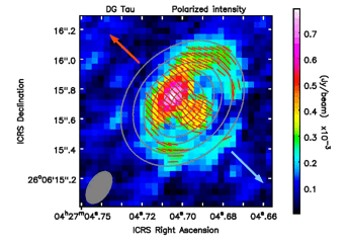
\includegraphics[width=6cm]{disco}
    %\caption{\footnotesize Disco stellare}
  \end{figure}
\end{minipage}
\begin{minipage}{0.6\textwidth}
  I parametri di Stokes sono molto importanti per gli astronomi. Infatti, ad esempio, nel caso di una stella in formazione con un ambiente intorno che sta collassando, questo si può vedere misurando la polarizzazione e notando come il disco è inclinato rispetto all'osservatore, quanto è grande il disco rispetto all'oggetto centrale, se questo ha una simmetria centrale ecc. 
\end{minipage}

\vspace{0.1cm}Calcoliamo per esercizio i parametri di Stokes in alcuni casi particolari di radiazione polarizzata linearmente:

\begin{itemize}
  \item Se la radiazione polarizzata oscilla verticalmente i parametri di Stokes saranno
  $$\begin{cases}
    I={E_{0y}}^2\\
    Q=-{E_{0y}}^2\\
    U=0\\
    V=0\\
  \end{cases}$$
  \item Se l'oggetto oscilla orizzontalmente saranno
  $$\begin{cases}
    I={E_{0x}}^2\\
    Q={E_{0x}}^2\\
    U=0\\
    V=0\\
  \end{cases}$$
  \item Quando l'oggetto oscilla sulla prima bisettrice, vale a dire $E_{0x}=E_{0y}$ e $\delta_1 -\delta_2=0$, si ha 
  $$\begin{cases}
    I=2{E_{0x}}^2\\
    Q=0\\
    U=2{E_{0x}}^2\\
    V=0\\
  \end{cases}$$
  mentre se oscilla nell'altra direzione, cioè con $\delta_1 -\delta_2=\pi$, otteniamo
  $$\begin{cases}
    I=2{E_{0x}}^2\\
    Q=0\\
    U=-2{E_{0x}}^2\\
    V=0\\
  \end{cases}$$
\end{itemize}

Il fatto che i parametri di Stokes sono così "strani" è legato al fatto che Poincaré ha eseguito dei calcoli di polarizzazione su una sfera, dove $Q$ e $U$ diventavano le coordinate sulla sfera.